%\documentclass[12pt,thmsa]{article}

\documentclass[11pt]{article}
\usepackage[spanish]{babel}  
\usepackage[utf8]{inputenc} 
\usepackage{amsmath}
\usepackage[pctex32]{graphicx}
\usepackage{amsfonts}
\usepackage{enumerate}
\usepackage{color}
\usepackage[normalem]{ulem} %%%% para tachar texto
\usepackage{setspace} %% interlineado
\usepackage{float}
\onehalfspacing

\usepackage{fouriernc} %%% Fuente más legible
\usepackage{merriweather} %%% Fuente más legible

\usepackage{geometry}
\geometry{
	a4paper,
	total={170mm,257mm},
	right=20mm,
	left=20mm,
	top=20mm,
	bottom=20mm
}

\title{\textbf{Teoría estadística de la información \\en el procesamiento de imágenes y señales}}
\date{}
\begin{document}
	
	\maketitle

%------------- Teoría de la información
En los últimos tiempos conceptos que provienen de la teoría de la información han sido utilizados para medir la desemejanza entre funciones de densidad. Especialmente el concepto de divergencia estocástica ha encontrado aplicaciones en áreas tan diversas como el procesamiento de señales e imágenes~\cite {Aviyente2007}, detección automática de regiones~\cite{Nascimento2009,SilvaCribariFrery:ImprovedLikelihood:Environmetrics}, clasificación de imágenes~\cite{Puig2003} entre otras aplicaciones. 
En Salicrú et al.~\cite{Salicru1994} los autores propusieron una familia de medidas de divergencia, llamadas $(h,\phi)$-divergencias que incluyen a la Kulback Leibler (KL) divergencia, a las $\phi$-divergencias presentadas por Csiszar~\cite{Csiszar1967} y a las generalizaciones de las $J$- divergencias y $R$-divergencias que fueron definidas por Taneja~\cite{Taneja1989} entre otras medidas. 

En la última década estas medidas han sido utilizadas en el procesamiento de imágenes adquiridas con radares de apertura sintética SAR. Estos sensores, que operan en el rango de microondas, tienen muchas aplicaciones debido a sus ventajas respecto de las imágenes que provienen de sensores ópticos. Dentro de las principales ventajas se encuentran la capacidad de proveer imágenes de alta resolución, y pueden operar en forma independiente de las condiciones climáticas y de la iluminación. Sin embargo, las imágenes SAR tienen la desventaja de ser difíciles de interpretar y analizar debido a la presencia del ruido speckle. Este ruido es inherente al proceso de captura de la imagen y se hace presente debido a la superposición coherente de las ondas reflejadas por
muchos dispersores. Esto causa una variación en la intensidad pixel a pixel que se manifiesta en la imagen como un patrón granular, por este motivo la utilización de modelos estadísticos es una herramienta esencial para describir este tipo de datos.

El modelo multiplicativo se ha utilizado con éxito para describir datos SAR. Se basa en la suposición de que el retorno $Z$ se puede describir como el producto de dos variables aleatorias independientes, $X\cdot Y$. La primera corresponde a la retrodispersión (la verdad no observada) y la segunda al ruido speckle~\cite{oliverquegan98}.

Frery et al.~\cite{Frery97} propusieron la familia de distribuciones $\mathcal{G}^0$ para modelar el retorno de imágenes SAR, este modelo es ampliamente utilizado porque tiene la capacidad de discriminar áreas con diferente grado de textura mejor que la familia de distribuciones $K$ como se indica en Mejail et al.~\cite{MejailJacoboFreryBustos:IJRS}.
Esta familia se describe por tres parámetros, el parámetro $\alpha$ que modela la textura, el parámetro $\gamma$ que informa sobre el brillo de la imagen y el número de looks $L$ que es proporcional a la relación señal/ruido. 
Debido a esta interpretación, la estimación de parámetros de calidad es de crucial importancia.

%%% ACF Esto parece repetido; si querés agregar algo, tendría que ir al principio
En los últimos tiempos se han utilizado medidas que provienen de la teoría de la información para extraer características en el procesamiento de imágenes SAR. 
Especialmente el concepto de divergencia estocástica ha encontrado aplicaciones en áreas tan diversas como el procesamiento de señales e imágenes~\cite {Aviyente2007}, detección automática de región en imágenes SAR~\cite{SilvaCribariFrery:ImprovedLikelihood:Environmetrics, Nascimento2009} entre otras aplicaciones.

En Cassetti et al.~\cite{APSAR2013ParameterEstimationStochasticDistances} los autores proponen un estimador mínima distancia para el parámetro de textura del modelo $\mathcal{G}^0$ minimizando una distancia estocástica entre el modelo teórico y una estimación no paramétrica de la función de densidad subyacente utilizando histogramas. En Gambini et al.~\cite{gambini2015} se estimó la función de densidad teórica del modelo $\mathcal{G}^0$  usando el kernel asimétrico Inverso Gaussiano (IG) con un ancho de banda elegido empíricamente. 
%%% ACF Sólo definir siglas y símbolos que se usan más de una vez
En Cassetti et al.~\cite{Cassetti2020} (artículo enviado para su publicación) se mejoró la propuesta mostrando que los núcleos asimétricos Lognormal (LN) y Gamma ($\Gamma$) tienen un mejor comportamiento que el IG en términos de error cuadrático medio integrado y se utilizó el método de validación cruzada de mínimos cuadrados (LSCV)~\cite{Rudemo1982} para la selección del ancho de banda en lugar de la selección empírica. Además se utilizó un algoritmo de búsqueda para encontrar el mínimo del estimador propuesto y se mostró que esta propuesta supera al estimador de máxima verosimilitud en cuanto a su robustez y tasa de convergencia.

Asimismo, Shannon~\cite{Shannon1948} propone una nueva manera de medir la transmisión de información a través de un canal, pensando a la información como un concepto estadístico. Propone como medida de información o de desorden a lo que se conoce como entropía de Shannon. En el caso discreto y considerando $X$ una variable aleatoria que toma $n$ valores con probabilidades $p_1,\ldots,p_n$, entonces la entropía de Shannon se define como $H(X)=-\sum_{i=1}^n p_i \log p_i$. Para el caso continuo se define $H(X)=-\int_{-\infty}^{\infty} f_X(x) \log f_X(x)$ donde $f$ es la función de densidad de probabilidad de la variable aleatoria $X$. Esta medida es un caso particular de las $(h,\phi)$ entropías propuestas por Salicrú et al.~\cite{salicruetal1993}.

En Ferreira et al.~\cite{Ferreira2020} se propone un nuevo método de segmentación para imágenes SAR polarimétricas basado en la entropía de Shannon. En Frery et al.~\cite{Frery2012} los autores encontraron expresiones explícitas para la entropía de Shannon y de Rényi para imágenes polarimétricas, y proponen medidas de contrastes basados en estas entropías. En~\cite{Rodrigues2016} los autores utilizaron un mapa de $\alpha$ estimado con el método Logcumulante propuesto por Nicolas et al. en~\cite{Nicolas2010}, como input para segmentar una imagen SAR monopolarimétrica modelada con la familia de distribuciones $\mathcal{G}^0$.

Varios autores propusieron estimadores para la entropía de Shannon, una revisión de estos métodos se puede encontrar en Beirlant et al.~\cite{Beirlant1997}. Recientemente Al-Omari~\cite{AlOmari2013} presentó nuevos estimadores para la entropía y Behmardi et.al~\cite{Behmardi2011} proponen un estimador paramétrico utilizando el principio de máxima entropía. 


%En la última década, los conceptos relacionados con la teoría de la información han ganado interés en el procesamiento de imágenes. Shannon~\cite{Shannon1948} definió la información $I(X,Y)$ entre las variables aleatorias $X$ e $Y$ como una divergencia calculada entre sus densidades de probabilidad.
%Se han propuesto varias medidas de divergencia para reflejar la cercanía entre dos funciones de distribución.
%Especialmente el concepto de divergencia estocástica ha encontrado aplicaciones en áreas tan diversas como el procesamiento de señales e imágenes~\cite {Aviyente2007}, detección automática de región en imágenes SAR~\cite{SilvaCribariFrery:ImprovedLikelihood:Environmetrics, Nascimento2009} entre otras aplicaciones.

%En Cassetti et al.~\cite{APSAR2013ParameterEstimationStochasticDistances} los autores proponen un estimador mínima distancia para el parámetro de textura del modelo $\mathcal{G}^0$ minimizando una distancia estocástica entre el modelo teórico y una estimación no paramétrica de la función de densidad subyacente utilizando histogramas. Los autores evaluaron diferentes distancias estocásticas y encontraron que la distancia triangular es la que mejor comportamiento presenta en términos de sesgo y error cuadrático medio. Gambini et al.~\cite{gambini2015} propusieron estimar $f$ usando el kernel asimétrico Inverso Gaussiano (IG) con un ancho de banda elegido empíricamente. En Cassetti et al.~\cite{Cassetti2020} artículo enviado para su publicación, se mejoró la propuesta mostrando que los núcleos asimétricos Lognormal (LN) y Gamma ($\Gamma$) tienen un mejor comportamiento que el IG en términos de error cuadrático medio integrado y se utilizó el método de validación cruzada de mínimos cuadrados (LSCV)~\cite{Rudemo1982} para la selección del ancho de banda en lugar de la selección empírica. Además se utilizó un algoritmo de búsqueda para encontrar el mínimo del estimador propuesto y se mostró que esta propuesta supera al estimador de máxima verosimilitud en cuanto a su robustez.

%Por otro lado, la teoría de la información ha sido aplicada a los métodos de estadística y probabilidades con éxito~\cite{Liese2006}. 
%Shannon~\cite{Shannon1948} definió la información $I(X,Y)$ entre las variables aleatorias $X$ e $Y$ como una divergencia calculada entre sus densidades de probabilidad. 
%Estas divergencias fueron ampliamente estudiadas por Kullback y Leibler~\cite{KullbackLeibler1951} y por Rényi~\cite{renyi1961} entre otros y es una medida de la distancia entre dos funciones de densidad. 

Asignar cada pixel de una imagen SAR a una clase es uno de los problemas fundamentales en la interpretación de este tipo de imágenes. Por este motivo clasificar la cobertura del suelo es uno de los objetivos principales en el análisis de datos provenientes de sensores remotos como son las imágenes SAR. Ésta se realiza con el objetivo de determinar áreas en la imagen con características comunes  y producir un mapa temático de la región donde las clases que se definen incluyen zonas urbanas, de pastura, agua, bosques, entre otras. En este sentido la clasificación de imágenes SAR juega un papel importante en muchos campos, como geología, agricultura entre otras disciplinas. En consecuencia, es de gran importancia el desarrollo de nuevas técnicas para interpretar los datos SAR con precisión y eficacia.

Los algoritmos de clasificación pueden dividirse en no supervisados y supervisados. En los primeros no se necesita que el clasificador interactúe con el usuario ya que éste realiza una búsqueda automática de grupos con características homogéneas dentro de la imagen. Los segundos requieren de muestras de entrenamiento definidas por el usuario con clasificación conocida, que serán utilizadas para clasificar pixeles con clasificación desconocida. En ambos algoritmos la extracción de características que permitan una clasificación precisa juega un rol de suma importancia.

Diferentes estrategias de clasificación no supervisadas se aplicaron a imágenes SAR. Carvalho et al.~\cite{Carvalho2019} implementaron algoritmos utilizando el conocido K-means junto con distancias estocásticas como medida de discimilaridad en imágenes PolSar. En~\cite{Fernandez2017} los autores aplicaron este tipo de clasificación basado en el algoritmo EM también en imágenes polarimétricas. 

Diversos algoritmos de clasificación supervisada han sido aplicados a imágenes SAR. En el trabajo de Akbarizadeh~\cite{Akbarizadeh2012} se aplicó el algoritmo Support Vector Machine (SVM) para clasificar una imagen SAR utilizando una nueva función de energía utilizando transformada wavelets. En Palacio et al.~\cite{Palacio2019} los autores combinaron la utilización de filtros con el algoritmo SVM en imágenes SAR polarimétricas para cuantificar el contenido de información basado en la precisión de la clasificación. En~\cite{Zhang2019} se propone un nuevo método de clasificación basado en redes neuronales. En~\cite{Parikh2020} se puede encontrar un review sobre métodos de clasificación para imágenes SAR.

%Como se señaló anteriormente, la principal diferencia entre los no supervisados ​​y supervisados
%enfoques es que los métodos no supervisados ​​no requieren que el usuario seleccione la capacitación
%conjuntos de datos para caracterizar los objetivos o entrenar al clasificador. En cambio, el usuario especifica
%solo el número de clústeres que se generarán, y el clasificador construye automáticamente
%los clústeres minimizando alguna función de error predefinida. A veces el número
%de grupos pueden ser detectados automáticamente por el clasificador (Cheung, 2005). En teoria,
%los usuarios no necesitan interactuar con el clasificador, que opera de forma independiente y
%automáticamente. Sin embargo, en la práctica, es más frecuente que los resultados sean aceptados.
%o rechazado en función de si cumplen o no con las expectativas del usuario.

%\citet{KullbackLeibler1951} (KL) estaban interesados en proponer una medida que discrimine dos poblaciones, considerando una cantidad que involucre medidas de informaci\'on. Su inter\'es era definir una magnitud que indique la diferencia entre dos funciones de distribuci\'on pensando en una generalizaci\'on de la entrop\'ia de Shannon. Si $p(x)$ y $q(x)$ son dos funciones de probabilidad puntual con el mismo soporte $\Omega$, la KL divergencia se define como $d_{\text{\tiny{KL}}}(p \rVert q)=-\sum_{x \in \Omega} p(x) \log \dfrac{q(x)}{p(x)}=\sum_{x \in \Omega} p(x) \log\dfrac{p(x)}{q(x)}$. 


%--------------- RUIDO
La formulación de nuevos métodos de filtrado de imágenes es un tema que está en continuo crecimiento, en particular para el caso donde el ruido no es gaussiano ni aditivo como es el ruido speckle. Los algoritmos NonLocalMeans (NLM), que inicialmente fueron propuestos por Buades et al.~\cite{Buades2005} en el contexto de modelos con ruido gaussino aditivo, utilizan la información que proveen los píxeles vecinos para estimar el valor del pixel en la imagen filtrada. El valor del pixel estimado se obtiene como un promedio ponderado donde el peso de cada pixel en la imagen original es proporcional a una medida de similitud entre los píxeles que se encuentran
un entorno ($E_1$) del pixel de referencia y los píxeles pertenecientes un entorno ($E_2$) de los alrededores de $E_1$. La figura~\ref{NLM} tomada de Penna et al.~\cite{Penna2013} muestra un esquema del funcionamiento de este algoritmo. 

\begin{figure}[hbt]
	\label{NLM}
	\centering
	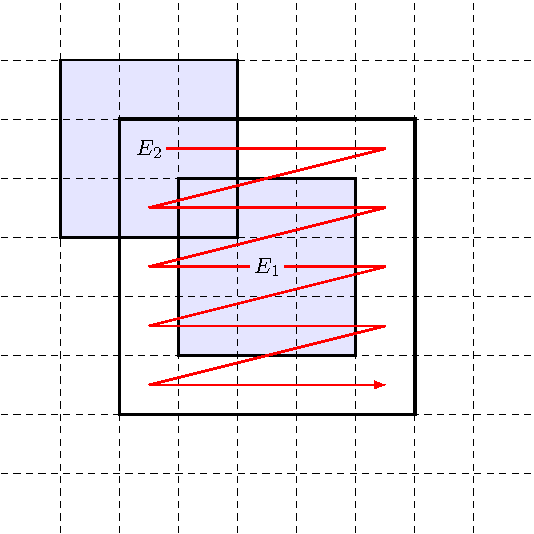
\includegraphics[scale=0.6]{../../Figures/Proyectos/UNGS2020/filtros.pdf}
	\caption{Funcionamiento del algoritmo NLM}
\end{figure}

Estos algoritmos proporcionan un marco general para el problema de reducción del ruido speckle dado que permiten proponer diferentes medidas de discimilaridad y diferentes pesos. En Penna et al.~\cite{Penna2013} los autores utilizaron la distancia de Kullback Leibler en imágenes SAR monopolarimétricas para datos de intensidad, en reemplazo de la distancia euclídea que se utiliza en el algoritmo NLM original. Esta idea fue tomada por Santos et al.~\cite{Santos2017} y los autores la aplicaron en imágenes de ultrasonido que también están afectadas por ruido speckle. En Xue et al.~\cite{Xue2013} los autores reemplazan a la función de peso en el algoritmo NLM original por una combinación lineal de funciones cosenos obteniendo un algoritmo más rápido. Un nuevo filtro basado en distancias estocásticas y test entre funciones de distribución fue porpuesto por Torres et al.~\cite{Torres2012} para datos SAR de intensidad.

Antes de proponer un método de clasificación hay que ser muy cuidadosos en elegir el modelo estadístico más apropiado y las características de la imagen que servirán de input para los algoritmos. Este proyecto estudiará la capacidad que tiene la entropía como característica de una imagen SAR en el contexto del diseño de nuevos métodos de filtrado y de clasificación de imágenes SAR.

\section{Objetivos generales}

%La hip´otesis general de este proyecto es que es posible proponer modelos
%estad´ısticos que describan los datos de las im´agenes adecuadamente, de tal
%forma que, combinados con m´etodos de segmentaci´on, y con estimaciones muy
%precisas de los par´ametros lleven a la formulaci´on de metodolog´ıas y al desarrollo
%de t´ecnicas para la extracci´on de conocimiento a partir de datos muy complejos
%como son las im´agenes SAR Polarim´etricas. De esta forma es posible obtener
%contornos de regiones muy bien definidos, lo que mejorar´ıa en gran medida la
%interpretaci´on autom´atica de la misma.


Este proyecto tiene como objetivo general profundizar en la utilización de medidas de discimilaridad que provienen de la teoría de la información que permitan tanto el desarrollo de nuevos métodos de clasificación basados en propiedades estadísticas del modelo considerado, como la implementación de nuevos métodos de filtrado de imágenes para la reducción del ruido speckle.

\section{Objetivos específicos}

Esta propuesta de investigación tiene por objetivos específicos:
\begin{itemize}
	\item Implementar distintos estimadores de la entropía para el modelo $\mathcal{G}^0$ para datos de intesidad.
	\item Evaluar la performance de estos estimadores para muestras de tamaño pequeño y moderado incluyendo el análisis bajo contaminación.
	\item Generalizar este estudio para entropías $(h,\phi)$ como las definidas en~\cite{Menendez1997} y~\cite{Salicru1994}. 
	\item Evaluar la performance de algoritmos de clasificación tanto supervisada como no supervisada, considerando a la entropía como atributo de la imagen.
	\item Obtener herramientas robustas que puedan ser implementadas en el diseño de procedimientos resistentes bajo contaminación tales como algoritmos de clasificación y filtros de la clase Nonlocal Means.
	\item Extender estos procedimientos diseñados para imágenes SAR para otras disciplinas como la Astroestadística.
	\item Fortalecer el vínculo generado entre la Universidad de Valparaíso, Universidad Federal de Alagoas y Universidad de Buenos Aires.
\end{itemize}

\section{Metodologías y fuentes}

Las imágenes SAR tienen muchas aplicaciones debido a sus ventajas respecto de las imágenes que provienen de sensores ópticos. La independencia de las condiciones climáticas y de la iluminación junto con la capacidad de penetrar la nubes, las copas de los árboles e incluso el suelo, han contribuido para que este tipo de imágenes resulten cada vez más populares.

Sin embargo, las imágenes SAR tienen la desventaja de ser difíciles de interpretar y procesar debido a la presencia del ruido speckle. Este ruido es inherente al proceso de captura de la imagen y se hace presente debido a la superposición coherente de las ondas reflejadas por muchos dispersores. Esto causa una variación en la intensidad pixel a pixel que se manifiesta en la imagen como un patrón granular. 

Debido a la aleatoriedad y a la fuerte dispersión que puede tener la señal retrodispersada, es necesario contar con modelos estadísticos que contribuyan a una mejor extracción de información a través del desarrollo de filtros, detección de bordes, clasificación de áreas entre otras metodologías. 

%El modelo multiplicativo es muy apropiado para explicar las características estadísticas de la imagen de un objeto cuando es iluminado por radiación coherente, como lo son las imágenes SAR.
%Este modelo considera que el valor observado en cada celda de la imagen es una variable aleatoria $Z$ que resulta del producto de dos variables aleatorias independientes: una correspondiente a la retrodispersión $X$ (que es lo que observaríamos sin la presencia del ruido speckle) y la otra correspondiente al ruido speckle $Y$ (que es inherente a todo sistema de captura de imágenes con iluminación coherente).

El modelo propuesto para datos provenientes de un sistema de iluminación por radiación coherente, como son los datos SAR, es un modelo multiplicativo que considera que el valor observado en cada celda de la imagen es una variable aleatoria $Z$ que resulta del producto de dos variables aleatorias independientes: una correspondiente al backscatter o retrodispersión $X$ (que es lo que observaríamos sin la presencia del ruido speckle) y la otra correspondiente al ruido speckle $Y$ (que es inherente a todo sistema de captura de imágenes con iluminación coherente). En los últimos años, se ha utilizado exitosamente la familia de distribuciones $\mathcal{G}^0$: $\mathcal{G}_A^0$ para datos de amplitud y $\mathcal G_I^0$ para datos de intensidad. Este modelo fue propuesto por Frery et al.~\cite{Frery97} y permite describir las áreas muy rugosas o extremadamente rugosas mejor que la distribución $\mathcal{K}$ como es presentado en \cite{Jakeman87}.

El modelo multiplicativo considerado es el siguiente:
\begin{equation*}
Z=X \cdot Y  
\end{equation*}
donde $X$ e $Y$ corresponden al backscatter y al ruido speckle, respectivamente. La variable aleatoria $Y$ se modela con la distribución $\Gamma ( L,L) $, donde $L\geq 1$ es el número de looks, mientras que $X$ sigue una distribución Gamma Inversa, denotada por  $\Gamma^{-1}(-\alpha ,\gamma) $. De esta forma tenemos que $Z$ obedece una distribución $\mathcal G_I^0$.

Su función de densidad está dada por
\begin{equation*}
f_{\mathcal{G}_I^{0}}( z) =\frac{L^{L}\Gamma ( L-\alpha
	) }{\gamma ^{\alpha }\Gamma ( -\alpha ) \Gamma (
	L) }\cdot  
\frac{z^{L-1}}{( \gamma +zL) ^{L-\alpha }},%
\label{ec_dens_gI0}
\end{equation*}
donde $-\alpha,\gamma ,z>0$ y $L\geq 1$.

Bajo este modelo se pueden caracterizar regiones con diferente grado de textura a través de los parámetros de la distribución $\mathcal{G}_I^{0}$. Para valores de $\alpha$ cercanos a cero (típicamente en el intervalo $(-3,0)$), la zona de la imagen corresponde a una región muy texturada, como es el caso de las zonas urbanas en las imágenes SAR. A medida que el valor del parámetro $\alpha$ disminuye, corresponde a zonas con cada vez menos textura, como son las regiones de forestación (usualmente $(-6,-3]$) y pastura (en $(-\infty,-6)$). Por otro lado, el parámetro $\gamma$ (llamado parámetro de escala) posee una interpretación en términos del brillo. Cuanto mayor es su valor, mayor intensidad posee la imagen en esa región. Por estas razones, la estimación precisa de los parámetros, en particular el parámetro de textura, es de suma importancia en el análisis de imágenes con ruido speckle. 

%En los últimos años se han propuesto varios métodos de estimación de parámetros, Vasconcellos et al.~\cite{VasconcellosFrerySilva:CompStat} cuantifican el error en la estimación del parámetro de textura para la distribución $\mathcal G_A^0$ y proponen una técnica analítica para mejorar la estimación.
%Silva et al.~\cite{SilvaCribariFrery:ImprovedLikelihood:Environmetrics} proponen otro método analítico para mejorar la estimación del parámetro de textura que reduce el error cuadrático medio.
%Cribari-Neto et al.~\cite{CribariFrerySilva:CSDA} proponen el uso de bootstrap para el mismo fin. 
%Allende et al.~\cite{AllendeFreryetal:JSCS:05} y Bustos et al.~\cite{BustosFreryLucini:Mestimators:2001} plantean mejoras para la estimación del parámetro de textura, pero con foco en su robustez. 

%Entre las técnicas de estimación paramétrica clásicas se encuentran las de máxima verosimilitud y momentos. Recientemente en~\cite{MellinAnalysisPolSAR,BujorTrouveValetNicolas2004,khan2014} han propuesto estimadores del parámetro de textura basado logcumulants y logmomentos, donde interviene la transforamda de Mellin de la función de densidad. En Tison et al.~\cite{Tison2004} los autores mostraron que los estimadors de los parámetros de la distribución $\mathcal G^0$, para datos de amplitud, mejoran al estimador de máxima verosimilitud.

Es importante contar con estimadores que tengan un comportamiento adecuado para muestras de pequeño y moderado tamaño tanto en sesgo, error cuadrático medio como en robustez. Esto es importante en el procesamiento de imágenes ya que muchos de los métodos de filtrado de imágenes, detección de bordes y clasificación utilizan máscaras deslizantes de tamaño $3 \times 3$,  $5 \times 5$, $7 \times 7$, $9 \times 9$ or  $11 \times 11$. 

Este proyecto se basa en la hipótesis general que consiste en considerar a otras medidas de discimiliardad, como son las $(h,\phi)$ entropías que, combinadas con la aplicación de filtros y métodos de clasificación permitan formular nuevas metodologías para la comprensión de imágenes SAR.

Este problema se abordará primeramente haciendo un relevamiento de los distintos estimadores de la entropía de Shannon como los propuestos en~\cite{Beirlant1997,AlOmari2013,Behmardi2011}. Teniendo en cuenta la expresión explícita de esta medida dada en Ferrerira et al.~\cite{Ferreira2020} para el caso de la función de densidad $\mathcal{G}_I^0$, y combinando con los resultados obtenidos en Cassetti et al.~\cite{Cassetti2020} en cuanto a la estimación del parámetro de textura, se implementarán estos estimadores y se estudiará la performance de los mismos a través de simulaciones Montecarlo donde se:
\begin{itemize}
	\item Considerará un espacio paramétrico que contemple distintas texturas, distintos números de looks y tamaño de muestra.
	\item Estudiará el sesgo, error cuadrático medio de los mismos.
	\item Analizará su robustez, es decir, su comportamiento bajo corrimientos del modelo teórico. 
	\item Evaluará su costo computacional.
\end{itemize} 

Se extenderá este estudio a otras entropías definidas dentro de la familia $(h,\phi)$ como las presentadas en~\cite{Frery2019}.

Un segundo paso es el diseño e implementación de nuevos procedimientos robustos para reducir la presencia del ruido speckle como, por ejemplo, los filtros NLM donde se propone como medida de distancia a la entropía. Se comparará el desempeño de esta propuesta con las existentes en la literatura a través de diferentes medidas como las que se indican en~\cite{Frery2019}.

Asimismo, algoritmos de clasificación serán estudiados para generar mapas temáticos de imágenes SAR utilizando medidas de discimilaridad. Estos algoritmos serán comparados con los existentes en la literatura a través de diferentes indicadores como los son el índice Kappa y la matriz de confusión.

%comparaci´on de los m´etodos de segmentaci´on basados en contornos combinados
%con la estimaci´on de los par´ametros
%
%Formulación de algoritmos para calcular nuevos estimadores de
%los par´ametros que sean robustos, implementaci´on computacional de los mismos
%y aplicaci´on a im´agenes sint´eticas y reales. Luego, medir el error que se comete
%al aplicarlos y comparar con diferentes m´etodos ya existentes en la literatura.
\bibliographystyle{plain}
\bibliography{../../Bibliography/bib_julia2}


\end{document}
